\documentclass[11pt,letter]{article}
\usepackage[top=1.00in, bottom=1.0in, left=1.1in, right=1.1in]{geometry}
\usepackage{Sweave}
\renewcommand{\baselinestretch}{1.1}
\usepackage{graphicx}
\usepackage{natbib}
\usepackage{amsmath}
\usepackage{xr-hyper}
\externaldocument{phencc}

\def\labelitemi{--}
\parindent=0pt

\begin{document}

\renewcommand{\refname}{\CHead{}}

\title{Supplemental materials:  How environmental tracking shapes species and communities in stationary and non-stationary systems} 

\author{E. M. Wolkovich \& M. J. Donahue}
\date{} 
\maketitle  %put the fancy title on
\renewcommand{\thetable}{S\arabic{table}}
\renewcommand{\thefigure}{S\arabic{figure}}


\section{Literature review}
We systematically reviewed the literature for studies examining tracking and other traits. We searched ISI in August 2019 for:
\begin{enumerate}
\item Topic: `phenolog* chang*' and Title: phenolog* AND trait*
\item Topic: `warming shift*' AND trait* and Title: phenolog*
\item Topic: `phenolog* track*' AND trait* and Title: phenolog*
\item Topic: `phenolog* sensitiv*' AND trait* and Title: phenolog*
\end{enumerate}
which resulted in 231 papers (83\% of which were published in 2011 or later, see Fig. \ref{fig:papertrends}). From here we used the following criteria to determine from which papers we could not extract data: no phenology or phenological change measured (73 papers), no trait(s) measured or analyzed (49 papers), single-species studies focused on intra-specific variation (55 papers), modeling or theory studies without data (12 papers), or papers without new data presented (reviews, etc.: 4 papers), or miscellaneous reasons leading to no data relevant to our aims (7 papers). This left us with 30 papers including relevant data \citep{Suzuki:1997gf,Post1999,adrian2006,Xu:2009an,Goodenough2010,Diamond:2011nx,Moussus2011,Szilvia2012,Dorji2013,Ishioka2013,xia2013,Bock2014,kharouba2014,Vegvari2015,bell2015,jing2016,lasky2016,McDermott2016,Zhu2016BioLetters,brooks2017,du2017,munson2017,arfinkhan2018,zhang2018,Ladwig2019,park2019,sharma2019,Xavier2019,Zettlemoyer2019}, nine of which did not test for a relationship between tracking and the other studied traits \citep{Suzuki:1997gf,adrian2006,Xu:2009an,Szilvia2012,bell2015,McDermott2016,Sherwood2017,sharma2019,Xavier2019}. We present data from the remaining papers in Tables \ref{tab:meta1}-\ref{tab:meta2}. \\

Most studies examined tracking as how a phenophase related to temperature (85\% of all tracking metrics), followed by precipitation (10\%, includes snow removal), followed by photoperiod (3\%), the climate mode NAO (1\%), water table depth (0.5\%), and year (0.5\%). Four of the 30 studies examined more than one major climate metric, though some measured many versions of temperature and/or precipitation metrics \citep[e.g., 15 precipitation and/or temperature metrics considered in][]{munson2017}.

% Could add why my review was not included (no tracking) and not including Brown review ... 
% Average number of traits and phenophases in each study. It was a mode of one for both phenophases and traits ... 

\newpage 
\clearpage
\section{Model} 
To give an example of how tracking and non-stationarity may be included in current models we modified a model from \citet{Chesson:2004eo}, which was originally conceptualized for annual plants with a seedbank.  Although the model can be conceived of more generally, we use the language of annual plant germination for concreteness. \\

The model includes a suite of species traits, including (and particularly relevant for our aims) traits controlling species response to the environment via germination each year and traits related to how species may bet-hedge across years (via a seedbank), as well as traits relating to resource competition each year. Within-season dynamics are controlled by resource competition resulting in fitness differences, while interannual variation in the environment provides opportunities for coexistence via fluctuation-dependent mechanisms (i.e., niche differences resulting from different germination functions). \\

Across years, for a community of \(n\) species, the seedbank ($N$) of species $i$ at time $t+1$ is determined by the survival ($s$) of seeds that did not germinate in last season ($1-g_{i}(t)$) plus new biomass ($B_i$) produced during the length of the growing season ($\delta$) converted to seeds at rate $\phi$:
\begin{align}
N_{i}(t+1) & =
s N_{i}(t)(1-g_{i}(t))+\phi B_{i}(t+\delta)
\end{align}
The production of new biomass each season follows a basic R* competition model: new biomass production depends on its resource uptake ($f(R)$ converted into biomass at rate $c_i$) less maintenance costs ($m$), with uptake controlled by $a$, $u$, and $\theta$:
\begin{align}
\frac{\mathrm{d}B_i}{\mathrm{d}t} & = c_{i}f(R) - m B_{i} \\
f(R) & = \frac{a R^{\theta}}{1+a uR^{\theta}}
\end{align}
With the initial condition:
\begin{align}
B_{i}(t+0) & = N_{i}(t)g_{i}(t)b_{0}
\end{align}
where $b_{0}$ is the initial biomass per seed.\\

The resource ($R$) itself declines across a growing season due to uptake by all species and abiotic loss ($\epsilon$):
\begin{align}
\frac{\mathrm{d}R}{\mathrm{d}t} & = - \sum_{i=1}^{n}f_{i}(R)B_{i} -\epsilon R
\end{align}
Germination depends both on the traits of the species and on the environment that year. The fraction of seeds germinating for a species each year is determined by the distance between $\tau_i$, a species characteristic, and $\tau_p(t)$, an attribute of the environment, which varies year-to-year.  Germination fraction declines according to a Gaussian as the distance between $\tau_i$ and $\tau_p(t)$ grows (we refer to this distribution as the `germination curve').  
%Need to add figure number!
\begin{align}
g_{i}(t) & = g_{max}e^{-h(\tau_{p}(t)-\tau_{i})^2} 
\end{align}

The model is designed for multiple conceptualizations \citep{Chesson:2004eo}; given our focus here, we consider $\tau_p(t)$ to represent the environmental (abiotic) start of the growing season that varies from year-to-year and refer to it as the `environmental start time.'  $\tau_i$ represents the `intrinsic biological start time' for species $i$. How well matched a species is to its environment each year can be measured as $\tau_i$-$\tau_p(t)$, or the distance between the intrinsic (biological) start time and the environmental start time. \\

\noindent \emph{Adding phenological tracking to model:}\\
We adjust the biological start time, $\tau_i$ so that it can respond to the environment dynamically through what we refer to as tracking. Tracking ($\alpha$, which can vary between 0 to 1) decreases the distance between $\tau_i$ and $\tau_p(t)$, i.e., moving the intrinsic start time closer to the environmental start time in that year, resulting in a higher germination fraction (e.g., species B in Fig. \ref{fig:concept}b-c).

\begin{align*}
\alpha_{i} & \in [0, 1]  
\end{align*}
\begin{align}
\hat{\tau_{i}} & = \alpha_{i} \tau_{p}(t) + (1-\alpha_{i})\tau_{i}
\end{align}
\noindent Thus, 
\begin{align*}
\text{when } \alpha_{i} = 0, & \hat{\tau_{i}}=\tau_{i}\\
\text{when }  \alpha_{i} = 1, & \hat{\tau_{i}}=\tau_{p}(t)
\end{align*}
% We refer to $\hat{\tau_{i}}$ as `effective biological start time' for species $i$ (or `effective $\tau_i$'). \\

\noindent \emph{Simulations:}\\
Using this model framework, we simulated a suite of two-species communities in stationary and non-stationary environments and examined persistence. As our interest is primarily in the role of environmental tracking, we focus on situations where species vary in their match to the environment through both the intrinsic biological start time ($\tau_i$) combined with tracking ($\alpha$), examining simulations where all species had some level of tracking. We also varied species' resource use efficiency (via $c_i$), yielding species with different $R^*$ (where a lower $R^*$ means a species can draw the resource down to a lower level and is thus considered the superior competitor). Each simulation was composed of two sequential parts: first, a 500-year stationary period where the underlying distribution of the environment does not change (but is stochastic, yielding year-to-year variation) followed by a 500-year non-stationary period where the underlying distribution of the environment shifts to an earlier start of season (see Fig. \ref{fig:modelfig} in main text). Thus, only species that persisted through the first stationary period continued into the non-stationary period.  \\

To simulate competitive dynamics, both species were initialized with a census size of $N(0) = 100$ per unit area, and the temporally varying parameters $R_0(t)$ and $\tau_{p}(t)$ were generated for the stationary and nonstationary periods. Species-specific parameters ($c_{i}$,$\tau_{i}$, and $\alpha_{i}$) were drawn from uniform random distributions with the ranges given in Table \ref{tab:model}.  All other parameters were identical between species (Table \ref{tab:model}).  Within-year $R^{*}$ competition dynamics were solved using an ode solver (\verb|ode| in the R package \verb|deSolve|) and ended when the resource was drawn down to $min(R^{*})$, i.e., the $R^{*}$ value of the better resource competitor.  The end of season biomass of each species was converted to seeds, and the populations were censused.  At each census, a minimum cutoff was applied to define extinction from the model.  Note that ``coexistence'' in this model is defined by joint persistence through time and not by low density growth rate. 

\section{References}
\bibliography{/Users/Lizzie/Documents/git/bibtex/LizzieMainMinimal}
\bibliographystyle{/Users/Lizzie/Documents/git/bibtex/styles/ecolett.bst}

\clearpage
\section{Tables \& figures}


\begin{center}
\begin{table}[h!]
\caption{Table of parameter values, definitions, and units.}
\begin{tabular}{ | p{2.0cm} | p{3.5cm} | p{5.0cm} | p{4.0cm} |}
\hline 
Parameter & Value(s) & Definition & Unit \\ \hline 
\(N_{i}\) & init cond $N_{i}(0) = 100; \n min(N_{i}(t)) = 10^{-4}$ & census of seedbank of species \(i\) & seeds per unit area \\ \hline
\(s\) & 0.8 & survival of species \(i\) & unitless \\ \hline
\(B_{i}\) & cf. Eqn 2 & biomass of species \(i\) & biomass \\ \hline
\(R_0\) & $\sim logN(\mu, \sigma)\n mu=log(2),\sigma = 0.2 $ & annually varying initial value of resource at the beginning of the growing season & resource\\ \hline
\(c_{i}\) & $\sim$Unif(8,20) & conversion efficiency of \(R\) to biomass of species \(i\) &  \(\frac{\text{biomass}}{\text{resource}}\) \\ \hline
\(m\) & 0.05 & maintenance costs during growth season \(i\) & \(\text{days}^{-1}\) \\ \hline
\(a\) & 20 & uptake increase as \(R\) increases for species \(i\) & \(\text{days}^{-1}\) \\ \hline
\(u\) & 1 & inverse of max uptake for species \(i\) & \(\frac{(\text{days})(\text{biomass})}{\text{resource}}\) \\ \hline
\(\theta\) & 1 & shape of uptake for species \(i\) & unitless\\ \hline
\(\phi\) & 0.05 & conversion of end-of-season biomass to seeds & \(\text{biomass}^{-1}\), but conceptually \(\frac{\text{seeds}}{(\text{biomass})(\text{seeds})}\) \\ \hline
\(\epsilon\) & 1 & abiotic loss of \(R\) &  \(\text{days}^{-1}\) \\ \hline
\(g_{max}\) & 0.5 & max germination rate of species & unitless \\ \hline
\(h\) & 100 &  controls the the rate at which germination declines as \(\tau_{p}\) deviates from optimum for species \(i\)  & \(\text{days}^{-2}\) \\ \hline
\(g_{i}\) & cf. Eqn 6 & germination rate & unitless \\ \hline
\(\tau_{p}\) & $\sim \beta(10,10)$ & timing of pulse & days \\ \hline
\(\tau_{i}\) & $\sim$ Unif(0.1,0.9) & timing of max germination of species \(i\) & days \\ \hline
\(\alpha_{i}\) & $\sim$ Unif(0,1) & phenological tracking of species \(i\) & unitless \\ \hline
\hline
\(b_{0}\) & 1 & biomass of a seedling & \(\frac{\text{biomass}}{\text{seeds}}\) \\ \hline
\(f(R)\) & cf. Eqn 3& resource uptake rate for species \(i\) & \(\frac{\text{resource}}{(\text{days})(\text{biomass})}\)\\ \hline
 \hline
\(t\) & 1 & annual timestep & years \\ \hline
\(0\) $\rightarrow$ \(\delta\) & determined by rate of resource depletion & time during the growing season & days \\ \hline
\hline
\end{tabular}
\label{tab:model}
\end{table}
\end{center}
\clearpage

 
\clearpage
% latex table generated in R 3.5.1 by xtable 1.8-3 package
% Thu Mar 19 12:34:53 2020
\begin{table}[ht]
\centering
\caption{Summary of traits related to phenological tracking in the literature and whether papers reported statistical evidence that they were linked or not. See Table S2 for an extended version.} 
\label{tab:meta1}
\begingroup\footnotesize
\begin{tabular}{lrr}
  \hline
Trait & n linked & n not linked \\ 
  \hline
diet traits &   0 &   3 \\ 
  early/late phenophase &  10 &   4 \\ 
  habitat traits &   1 &   3 \\ 
  height &   1 &   0 \\ 
  hibernation stage &   0 &   3 \\ 
  leaf/shoot size &   1 &   0 \\ 
  migration traits &   3 &   2 \\ 
  mobility &   1 &   3 \\ 
  nativeness &   1 &   3 \\ 
  niche breadth &   3 &   2 \\ 
  other Lepidopteran traits &   3 &   4 \\ 
  other bird traits &   1 &   1 \\ 
  other leaf traits &   4 &   3 \\ 
  other plant traits &   1 &   1 \\ 
  overwintering &   2 &   1 \\ 
  range traits &   1 &   4 \\ 
  root traits &   3 &   0 \\ 
  seed weight/size/number &   1 &   2 \\ 
  woody/herbaceous &   1 &   0 \\ 
   \hline
\end{tabular}
\endgroup
\end{table}% latex table generated in R 3.5.1 by xtable 1.8-3 package
% Thu Mar 19 12:34:53 2020
\begin{table}[ht]
\centering
\caption{Summary of results from literature on phenological tracking showing which phenophases researchers found were linked to which traits, or not.} 
\label{tab:meta2}
\begingroup\footnotesize
\begin{tabular}{lllrr}
  \hline
Taxa & Phenophase & Trait & n linked & n not linked \\ 
  \hline
Lepidoptera & activity length & hibernation stage &  &   1 \\ 
  Lepidoptera & activity length & migration traits &  &   1 \\ 
  Lepidoptera & activity length & other Lepidopteran traits &   1 &  \\ 
  Lepidoptera & appearance/collection date & diet traits &  &   1 \\ 
  Lepidoptera & appearance/collection date & early/late phenophase &   2 &  \\ 
  Lepidoptera & appearance/collection date & habitat traits &  &   2 \\ 
  Lepidoptera & appearance/collection date & hibernation stage &  &   1 \\ 
  Lepidoptera & appearance/collection date & migration traits &   1 &  \\ 
  Lepidoptera & appearance/collection date & mobility &  &   2 \\ 
  Lepidoptera & appearance/collection date & niche breadth &   2 &   1 \\ 
  Lepidoptera & appearance/collection date & other Lepidopteran traits &   1 &   2 \\ 
  Lepidoptera & appearance/collection date & overwintering &   2 &  \\ 
  Lepidoptera & appearance/collection date & range traits &   1 &   2 \\ 
  Lepidoptera & flight timing & early/late phenophase &   1 &   1 \\ 
  Lepidoptera & flight timing & mobility &   1 &   1 \\ 
  Lepidoptera & flight timing & niche breadth &  &   1 \\ 
  Lepidoptera & flight timing & other Lepidopteran traits &  &   1 \\ 
  Lepidoptera & flight timing & overwintering &  &   1 \\ 
  Lepidoptera & flight timing & range traits &  &   1 \\ 
  Lepidoptera & last/median emergence dates & diet traits &  &   1 \\ 
  Lepidoptera & last/median emergence dates & habitat traits &  &   1 \\ 
  Lepidoptera & last/median emergence dates & hibernation stage &  &   1 \\ 
  Lepidoptera & last/median emergence dates & migration traits &  &   1 \\ 
  Lepidoptera & last/median emergence dates & other Lepidopteran traits &   1 &   1 \\ 
  passerine birds & breeding time & diet traits &  &   1 \\ 
  passerine birds & breeding time & habitat traits &   1 &  \\ 
  passerine birds & breeding time & migration traits &   2 &  \\ 
  passerine birds & breeding time & niche breadth &   1 &  \\ 
  passerine birds & breeding time & other bird traits &   1 &   1 \\ 
  plants & budbreak/leafing & early/late phenophase &   3 &   1 \\ 
  plants & budbreak/leafing & nativeness &  &   1 \\ 
  plants & budbreak/leafing & other leaf traits &   2 &   1 \\ 
  plants & budbreak/leafing & range traits &  &   1 \\ 
  plants & flowering/fruiting & early/late phenophase &   4 &   2 \\ 
  plants & flowering/fruiting & height &   1 &  \\ 
  plants & flowering/fruiting & leaf/shoot size &   1 &  \\ 
  plants & flowering/fruiting & nativeness &   1 &   2 \\ 
  plants & flowering/fruiting & other leaf traits &   2 &   2 \\ 
  plants & flowering/fruiting & other plant traits &   1 &   1 \\ 
  plants & flowering/fruiting & root traits &   3 &  \\ 
  plants & flowering/fruiting & seed weight/size/number &   1 &   2 \\ 
  plants & flowering/fruiting & woody/herbaceous &   1 &  \\ 
   \hline
\end{tabular}
\endgroup
\end{table}

\clearpage
\begin{figure}[t!]
\centering
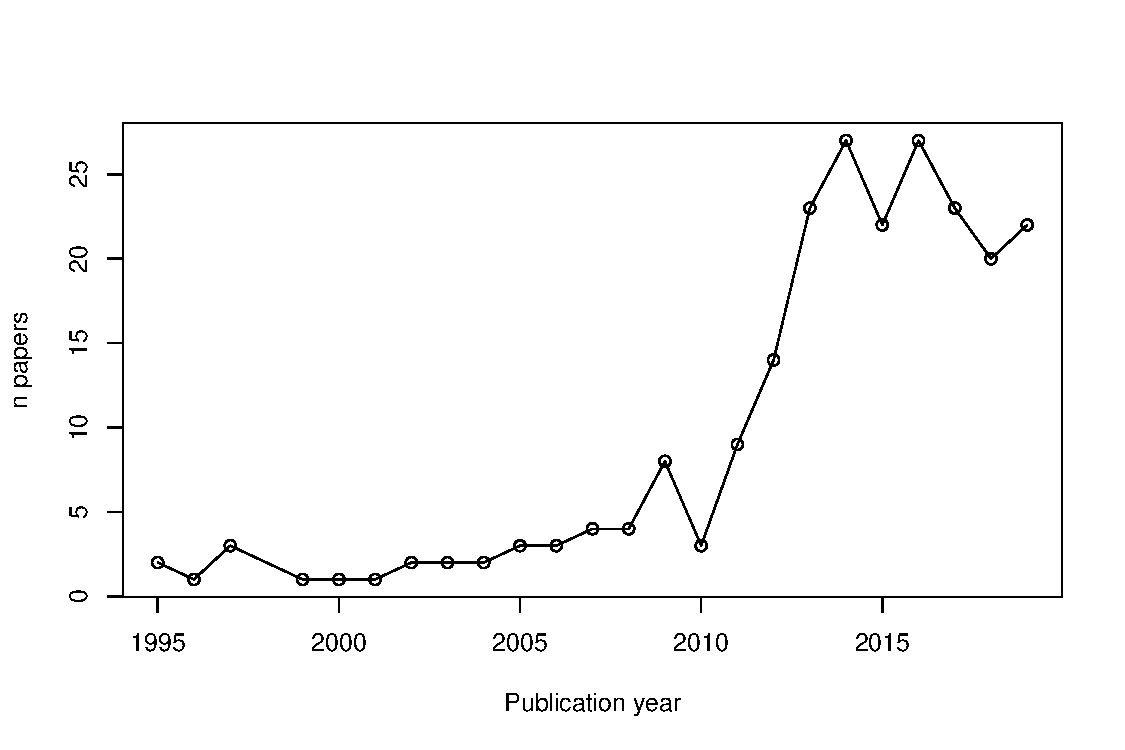
\includegraphics[width=1\textwidth]{..//..//..//R/graphs/otherdat/papersovertime.pdf}
\caption{Trends in all papers using search terms over time. Of papers from which we could extract data all 25 of 30 were published in 2011 or onward.}
  \label{fig:papertrends}
\end{figure}

\begin{figure}[t!]
\centering
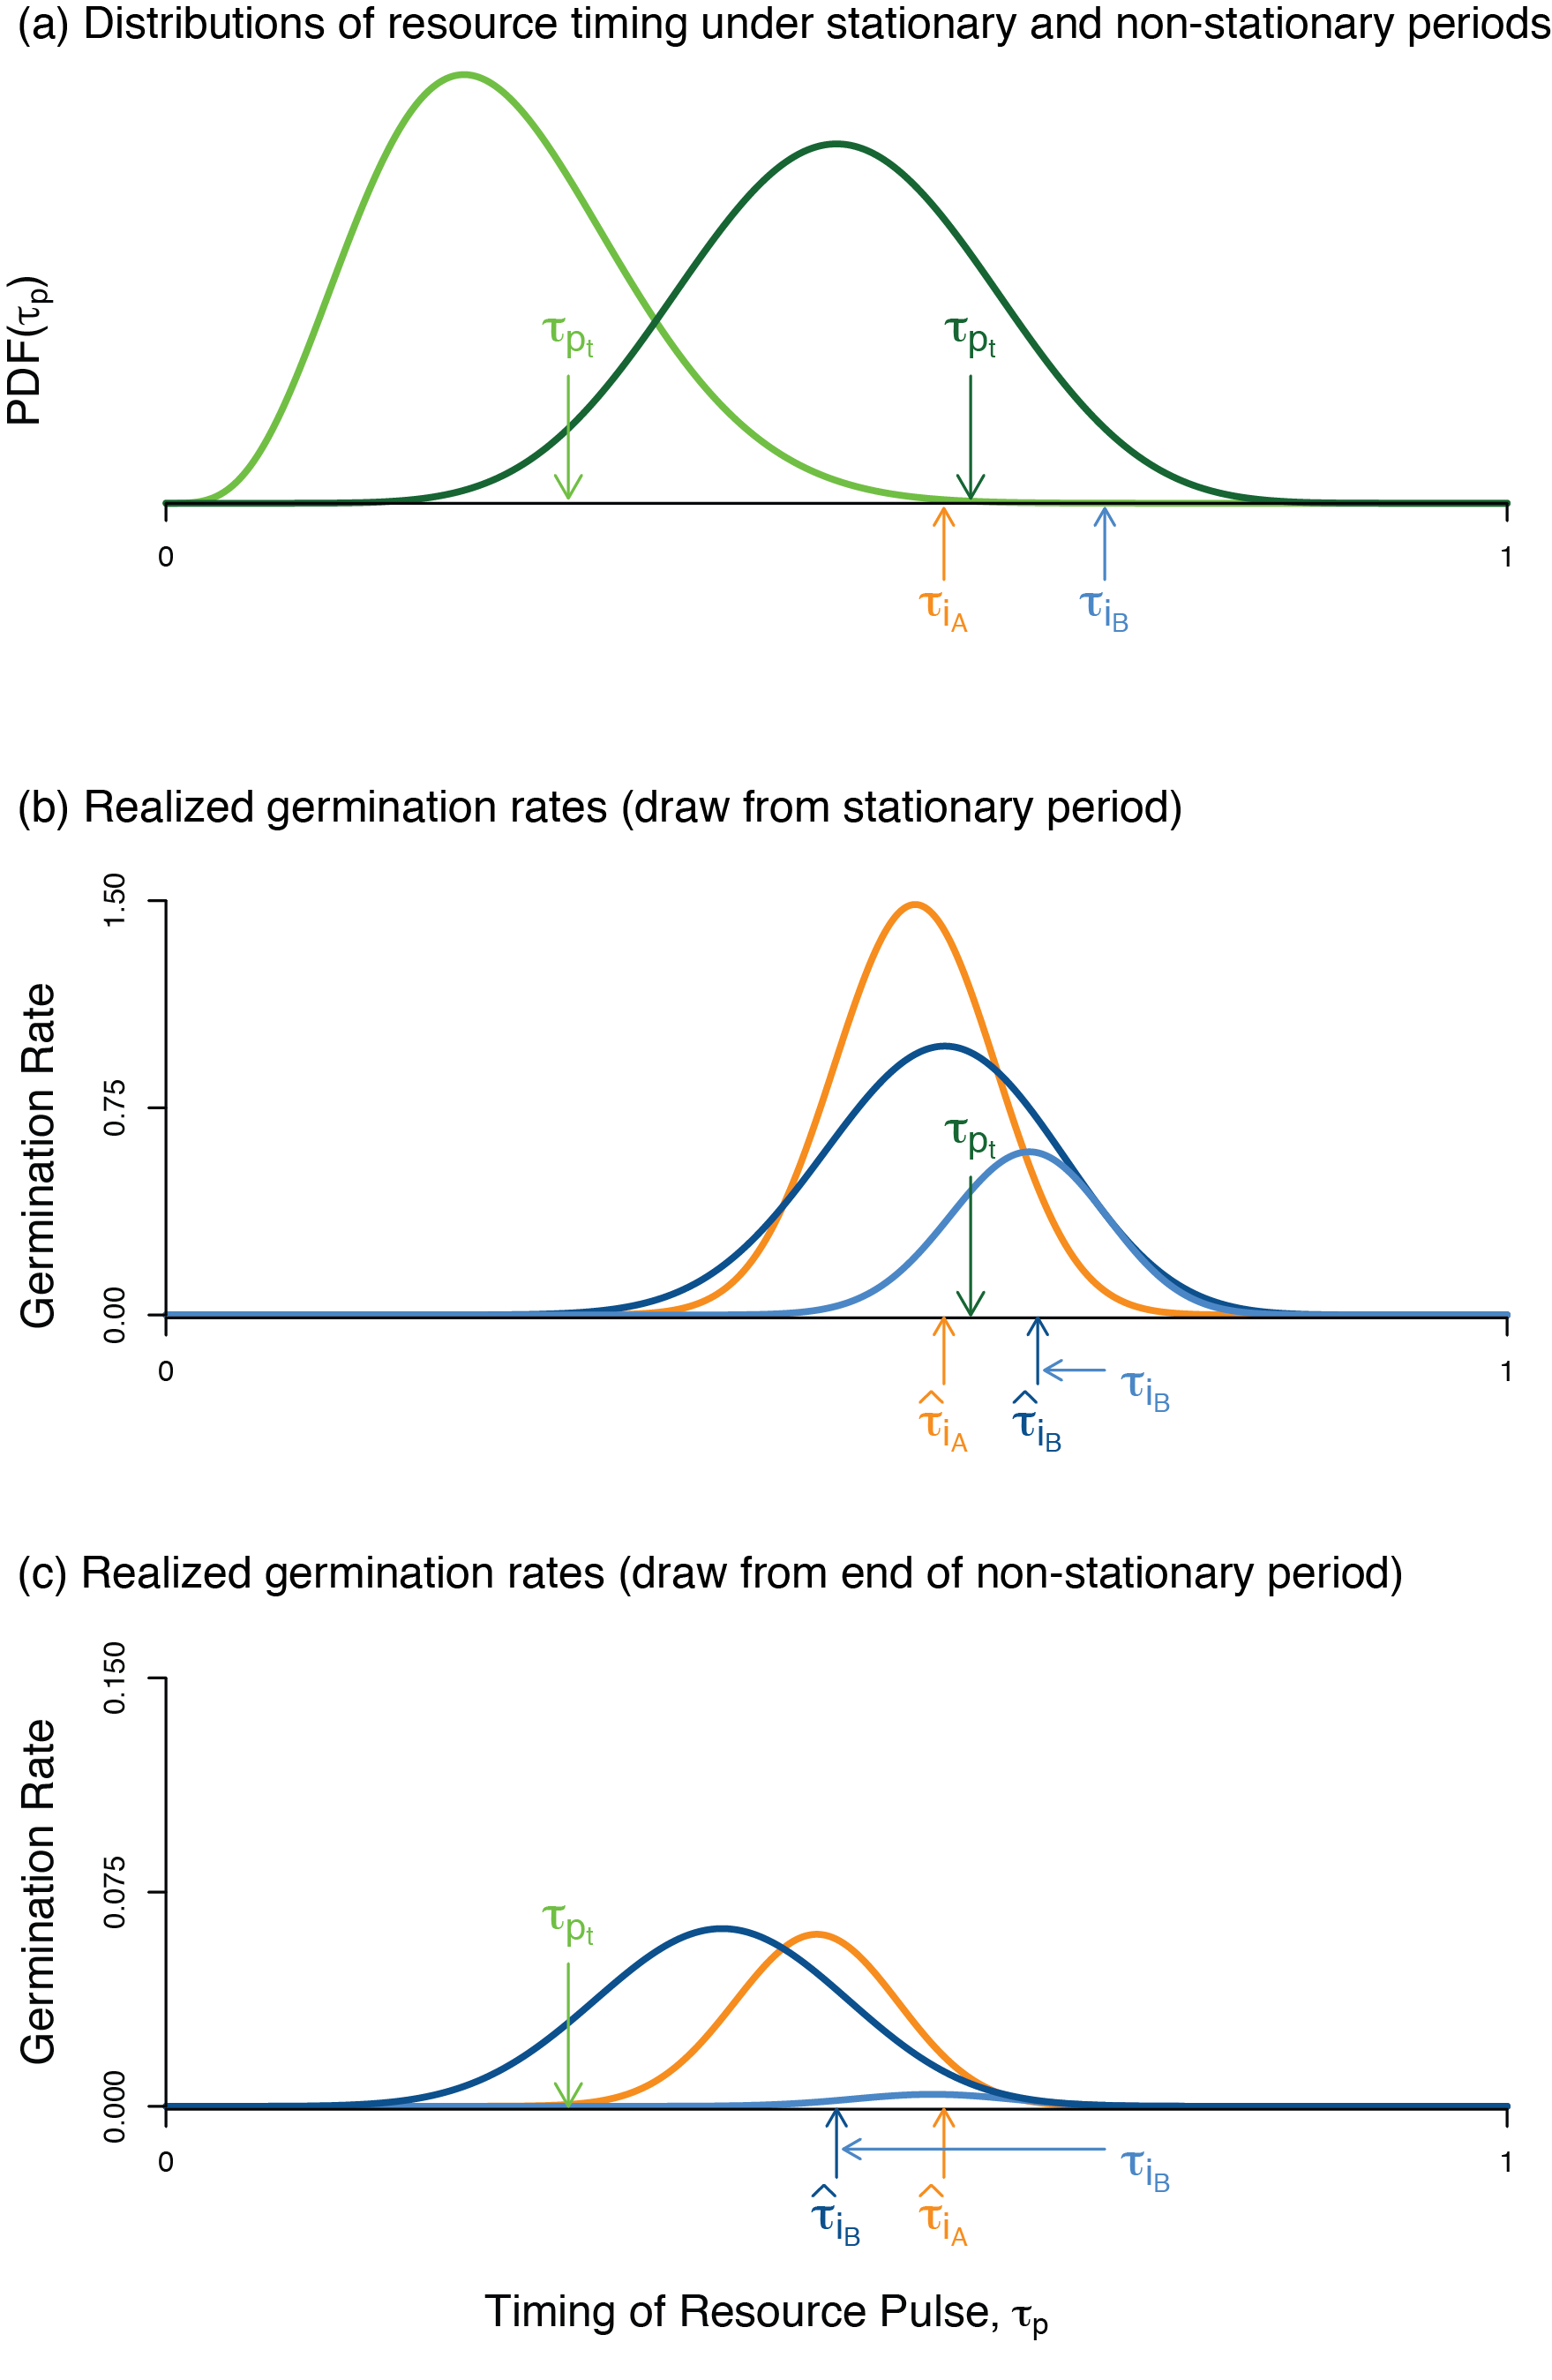
\includegraphics[width=0.65\textwidth]{..//..//..//R/graphs/conceptual/TauP_GerminationAdj.png} 
\caption{The distributions of the environment (a) and species' germination for two sample years (b-c) in our seed germination model. (a) The timing of the resource pulse ($\tau_p(t)$), which defines the environmental start of season, is $\beta$-distributed with parameters $\beta(10,10)$ during the stationary period (dark green) shifting to $\beta (5,15)$ through the nonstationary period (light green). (b) Realized germination rate as a function of $\tau_p(t)$ for two species during the stationary period: the orange line is a non-tracking species A with preferred germination time, $\tau_{iA}$, that is close to the mean of the stationary period; the blue lines show the difference in realized germination rate of a tracking species with a preferred germination time, $\tau_{iB}$, that is further from the mean of the stationary period both without (light blue) and with (dark blue) the effect of tracking; note the shift from $\tau_{iB}$ to $\hat{\tau_{iB}}$. (c) Realized germination rate of species A and species B at the end of the nonstationary period. Note the change in axes from (b) to (c) shows the decline in overall germination rate as the environment moves away from the preferred germination time of both species.} % I'm not sure that "realized germiantion" is the best phrase, but it is the germination rate given tauP times the prob of tauP under that STA or NST period.  So it it he realized germination rate for each species given the environment.  
% If, in a particular year, $\tau_i$ is close to $\tau_p$, a large fraction of species $i$ seeds will germinate (e.g., Fig. \ref{fig:concept}b) ; if $\tau_i$ is far from $\tau_p$, a small fraction of the seeds will germinate.  Figure \ref{fig:concept} b-c illustrate the germination rate of two species with different $\tau_i$ values under two different environments.   
\label{fig:concept}
\end{figure}

\iffalse % tauI figures commented out just now
\begin{figure}[t!]
\centering
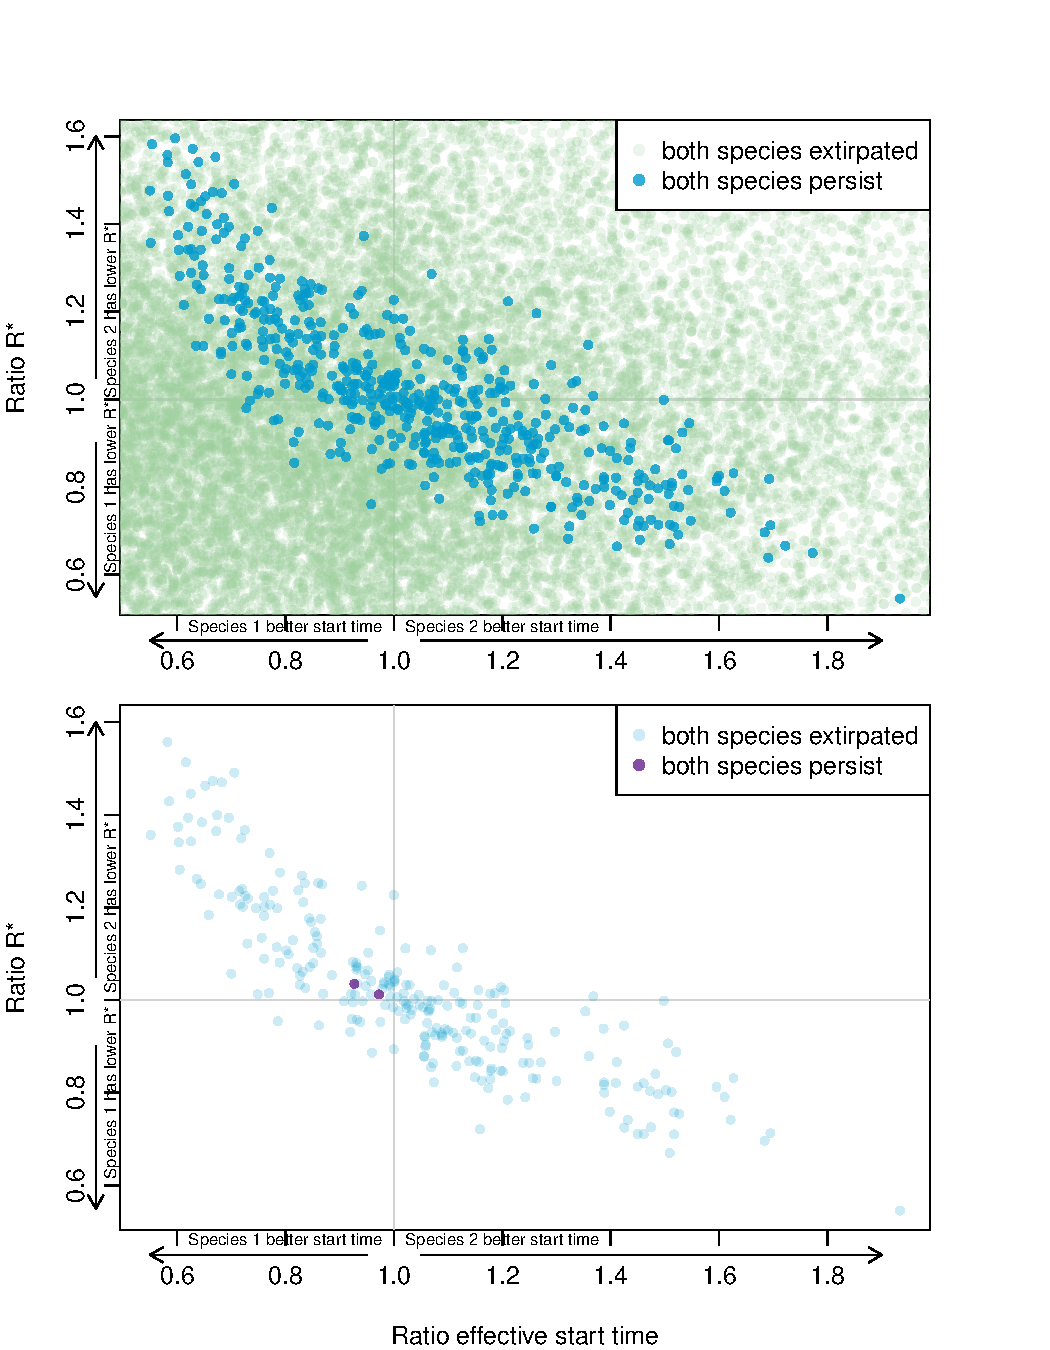
\includegraphics[width=0.9\textwidth]{..//..//..//R/graphs/modelruns/manuscript/tauIPrstart1_2panel.pdf}
\caption{How non-stationarity reshapes two-species communities in a simple model where effective start time (X axis: species 1/species 2) trades off with $R^*$ (Y axis: species 1/species 2): each point represents one two-species community color-coded by whether both species persisted or one or more species was extirpated through 500 years of a stationary environment (top), followed by an additional 500 years of non-stationary environment (bottom), where the abiotic start of the season shifts earlier. Only two-species communities that persisted through the stationary period are shown in the bottom panel. See Fig. \ref{fig:tauirstarsupp} for an alternative version of this figure detailing one-species outcomes.}
 \label{fig:tauirstar}
\end{figure}
\clearpage

\begin{figure}[t!]
\centering
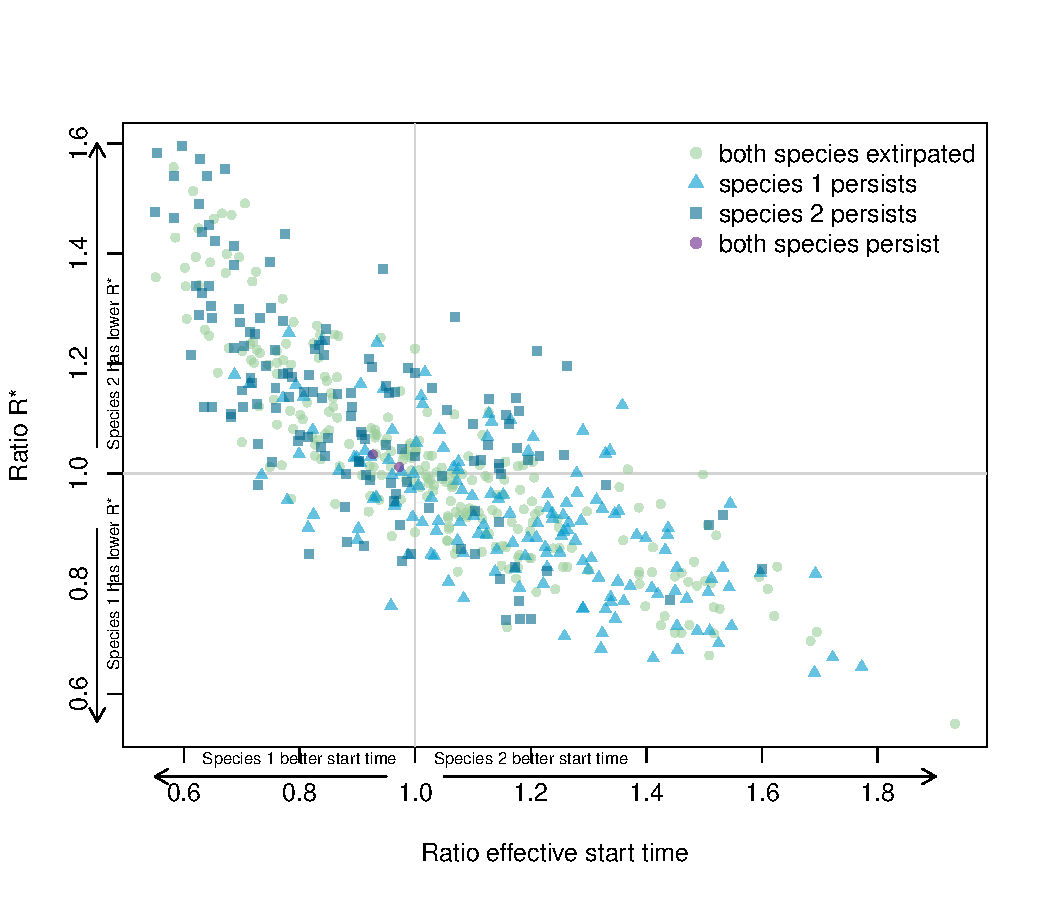
\includegraphics[width=0.9\textwidth]{..//..//..//R/graphs/modelruns/manuscript/tauIPrstart1.pdf}
\caption{How non-stationarity reshapes two-species communities in a simple model where effective start time (X axis: species 1/species 2) trades off with $R^*$ (Y axis: species 1/species 2): each point represents one two-species community that persisted through 500 years of stationary dynamics while the shape and color represent the outcome for that two-species community of 500 years of non-stationarity, where the abiotic start of the season shifts earlier.}
 \label{fig:tauirstarsupp}
\end{figure}
\fi

\begin{figure}[t!]
\centering
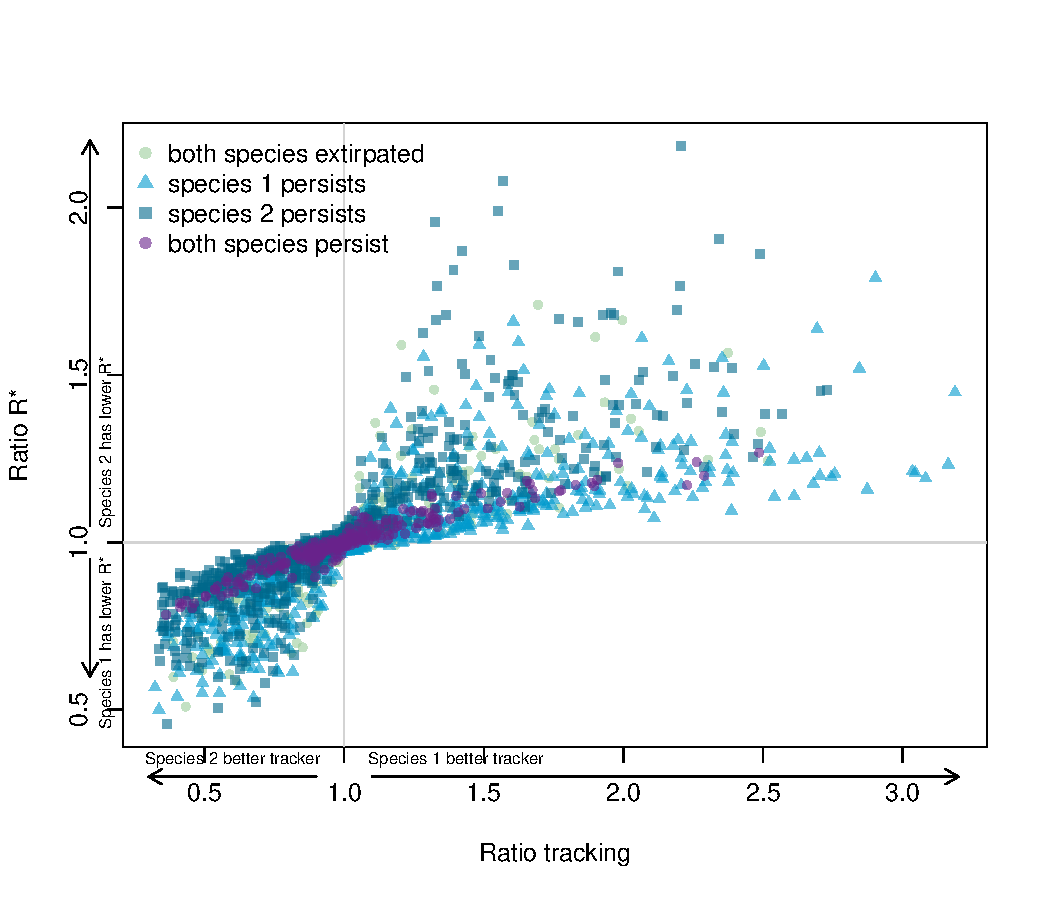
\includegraphics[width=0.9\textwidth]{..//..//..//R/graphs/modelruns/manuscript/alpharstar.pdf}
\caption{How non-stationarity reshapes two-species communities in a simple model where tracking (X axis: species 1/species 2) trades off with $R^*$ (Y axis: species 1/species 2): each point represents one two-species community that persisted through 500 years of stationary dynamics while the shape and color represent the outcome for that two-species community of 500 years of non-stationarity, where the abiotic start of the season shifts earlier.}
\label{fig:alpharstarsupp}
\end{figure}

\end{document}




% All in PhenologyModelFigSupp.R ... not sure why it would not work! Worked if you put it towards top of file. 
 
